\section*{Problema 5.1}
Dado $\lambda = 633nm$, $P = 0.01pW$ y una eficiencia $\eta = 30\%$ a intervalos de $10ms$. Se tiene
\begin{enumerate}[a)]
	\item La tasa de conteo en términos del flujo de fotones $\phi = \flatfrac{P\lambda}{hc} = 31843.9\text{fotones}/s \approx 3.2\times 10^{4} \text{fotones}/s$,
		$$ \mathcal{R} = \eta \phi \approx \boxed{ 9600 \text{count}\, s^{-1}. } $$
	\item El promedio de conteos
		$$ N(T) = \mathcal{R} T = 0.01*9600 = \boxed{ 96. } $$
	\item La desviación estandar definida por $\Delta n = \sqrt{\bar{n}} = \sqrt{N(T)}$, se tiene
		$$ \Delta n = \boxed{ 9.79795 \approx 10. } $$
\end{enumerate}


\section*{Problema 6.1}
Para este problema, se realizó una figura representando el problema y la equivalencia entre los ánulos $\theta _1$ y $\theta _2$.

\begin{figure}[H]
	\centering
	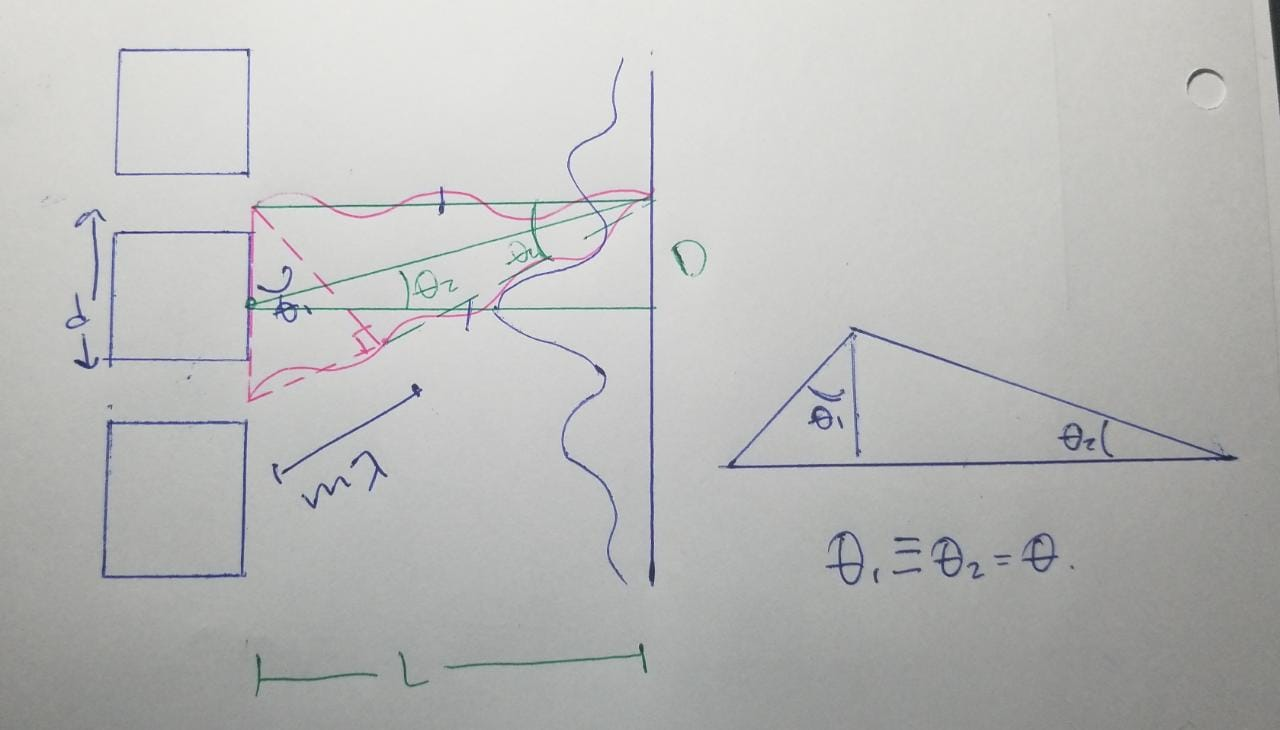
\includegraphics[scale=0.25]{img/6_1.jpeg}
	\caption{Representación gráfica del experimento de doble rendija. El término $m\lambda$ representa las $m$ longitudes de onda de diferencia entre cada 'rayo', por características del problema $m = 1$. Además, dadas las relaciones trigonométricas para el triángulo rectángulo se tiene $\sin{\theta _1} = \flatfrac{m\lambda}{d}$ y $\tan{\theta _2} = \flatfrac{D}{L}$.}
	\label{6_1}
\end{figure}


Con esto, se tienen dos representaciones distintas de $\theta$
\begin{align}
	\sin{\theta} &= m\frac{\lambda}{d}, \label{theta1} \\
	\tan{\theta} &= \frac{D}{L}. \label{theta2}
\end{align}
Dado que $D\ll L$, entonces $\tan{\theta} \approx \sin{\theta} \approx \theta$, entonces
	$$ \theta = \frac{D}{L} = \frac{\lambda}{d} \qquad \Rightarrow \qquad \boxed{\frac{D}{L} = \frac{\lambda}{d}. } $$



\section*{Problema 7.6}
Sabiendo que $\abs{\alpha} = \sqrt{\bar{n}}$, con $\alpha = 5$, se tiene	
\begin{enumerate}[a)]
	\item Promedio de número de fotones
		$$ \bar{n} = \boxed{ 25. } $$
	\item Desviación estandar
		$$ \Delta n = \abs{\alpha} = \boxed{ 5. } $$
	\item La incerteza de fase
		$$ \Delta \phi = \frac{1}{2\sqrt{\bar{n}}} = \boxed{ 0.1 rad. } $$
\end{enumerate}


\section*{Problema 7.7}
Dado el laser que emite pulsos de energía $1mJ$ y longitud de onda $693nm$, entonces se tiene $E = n\frac{hc}{\lambda}$
	$$ n = \frac{E\lambda}{hc} = 3486\times 10^{15}; $$
por lo que, la incerteza de fase es
	$$ \Delta \phi = \frac{1}{2\sqrt{n}} = \boxed{ 8.468\times 10^{-9}. } $$



















%%%%%